\documentclass{article}
\usepackage{import}
\usepackage{amsmath}
\usepackage{tabularray}
\usepackage{float}


\import{lib/latex/}{wgmlgz}
\patchcmd{\thebibliography}{\section*}{\section}{}{}

\begin{document}
\itmo[
      variant=13,
      labn=6,
      discipline=Вычислительная математика,
      group=P3212,
      student=Соколов Анатолий Владимирович,
      teacher=Наумова Надежда Александровна 
]
\lstset{language=rust}
\newgeometry{
  a4paper,
  top=20mm,
  right=10mm,
  bottom=20mm,
  left=30mm
}
\tableofcontents
\section{Задание}
      \subsection{Порядок выполнения работы}
      	\begin{enumerate}
			\item В программе численные методы решения обыкновенных дифференциальных уравнений (ОДУ) должен быть реализован в виде отдельного класса /метода/функции;
			\item Пользователь выбирает ОДУ вида $y^\prime=f(x,y)$ (не менее трех уравнений), из тех, которые предлагает программа;
			\item Предусмотреть ввод исходных данных с клавиатуры: начальные условия $y_0=y(x_0)$, интервал дифференцирования $[x_0,x_n]$, шаг $h$, точность $\varepsilon$;
			\item Для исследования использовать одношаговые методы и многошаговые методы (см. табл.1);
			\item Составить таблицу приближенных значений интеграла дифференциального уравнения, удовлетворяющего начальным условиям, для всех методов, реализуемых в программе;
			\item Для оценки точности одношаговых методов использовать правило Рунге;
			\item Для оценки точности многошаговых методов использовать точное решение задачи: $\varepsilon = \max_{0\leq i \leq n}|y_{i \text{точн}}-y_i|$
			\item Построить графики точного решения и полученного приближенного решения (разными цветами);
			\item Программа должна быть протестирована при различных наборах данных, в том числе и некорректных.
			\item  Проанализировать результаты работы программы.
     	\end{enumerate}       
\subsection{Вариант}
      \subsubsection{Методы для реализации в программе:}
            Одношаговые методы:
            \begin{enumerate}
                  \item Метод Эйлера,
                  \item Усовершенствованный метод Эйлера,
                  \item Метод Рунге-Кутта 4- го порядка.
            \end{enumerate}
            Многошаговые методы:         
            \begin{enumerate}
            	\setcounter{enumi}{3}
            	\item Адамса
            	\item Милна
            \end{enumerate}
            \begin{table}[H]
                  \begin{tabular}{|l|l|}
                        \hline
                        № варианта & метод \\ \hline
                        13 & 1,2,5 \\ \hline
                  \end{tabular}
                  \caption{\small \sl {Таблица 1.2}} 
            \end{table}
\subsection{Цель работы}
      Решить задачу Коши для обыкновенных дифференциальных уравнений численными методами.



\section{Выполнение}            
      \subsection{Блок-схема реализованного алгоритма}
		\begin{figure}[H]
    		\centering
    		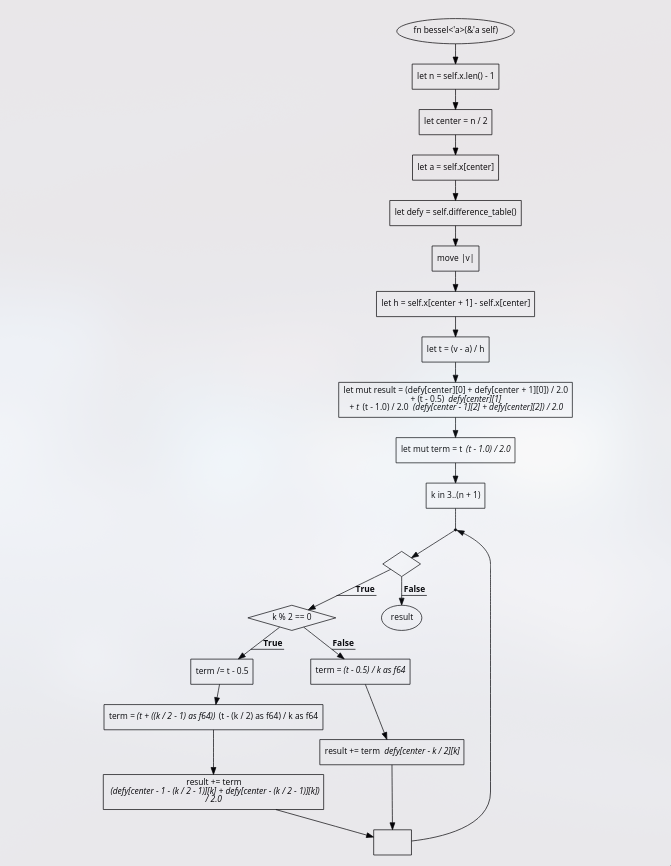
\includegraphics[width=360pt]{alg5.png}
    		\caption[Схема-1]{Метод Бесселя}
    		\label{fig:screenshot003}
    	\end{figure}             
      \subsection{Ссылка на GitHub c основной реализацией}
            \href{https://github.com/isofinly/compmath}{Github}

      \subsection{Примеры и результаты работы программы}
            \begin{figure}[H] 
                  \begin{center}  
                        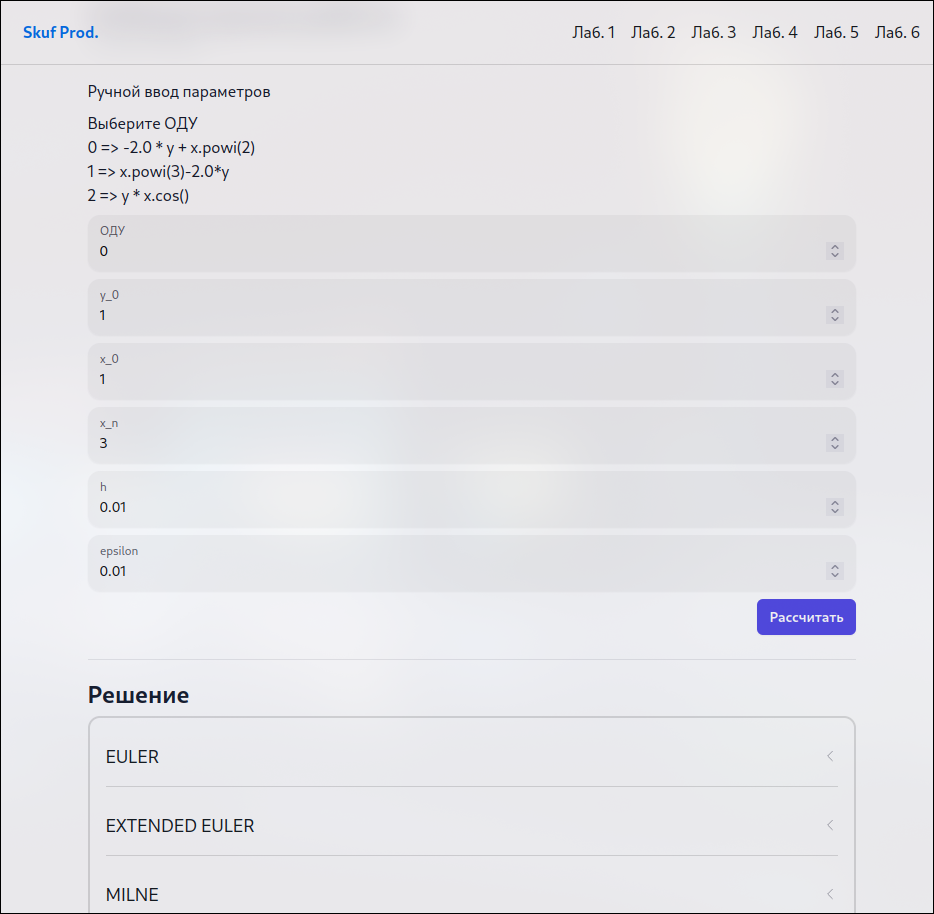
\includegraphics[scale=0.4]{ui1.png}
                        \caption{\small \sl {UI  1}}  
                  \end{center}  
            \end{figure}
             \begin{figure}[H] 
            	\begin{center}  
            		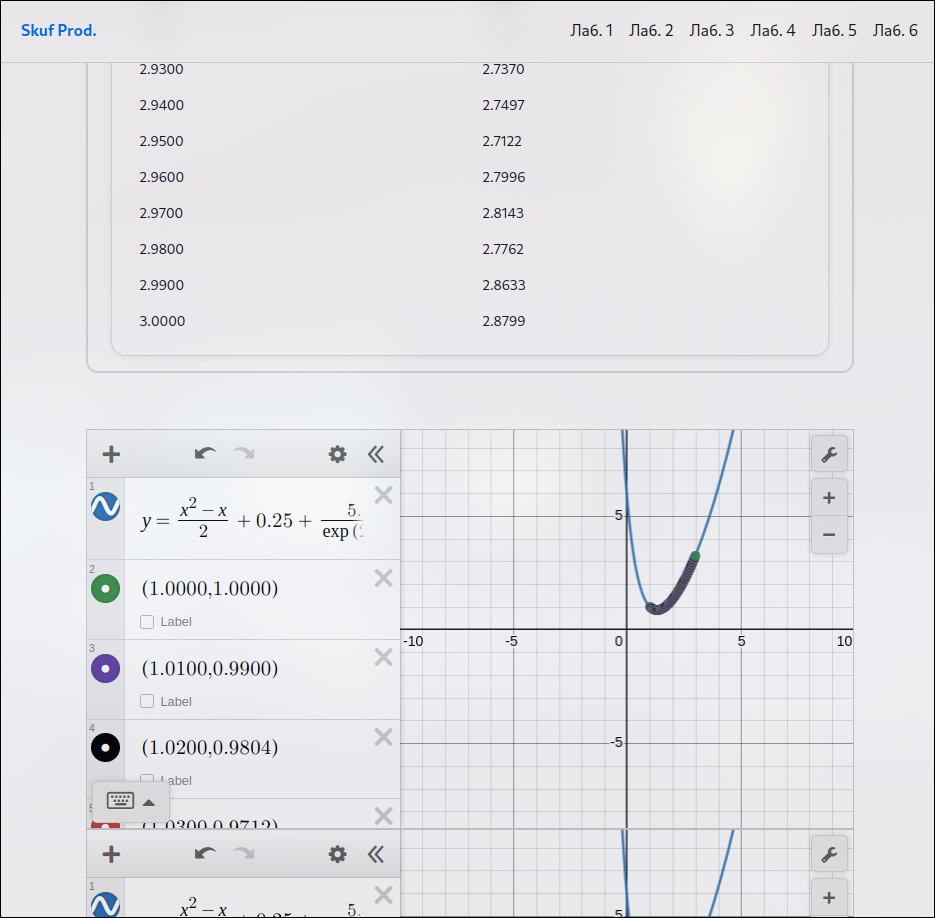
\includegraphics[scale=0.4]{ui2.png}
            		\caption{\small \sl {UI  1}}  
            	\end{center}  
            \end{figure}
            
\section{Заключение}
      В ходе выполнения данной ЛР я ознакомился с основыми методами решения ОДУ. Вообще с кайфом написал программу и посчитал ручками.

\begin{thebibliography}{9}
    \bibitem{Методичка}Слайды с лекций (2023). // Кафедра информатики и вычислительной техники -- Малышева Татьяна Алексеевна, к.т.н., доцент.
\end{thebibliography} 

\end{document}
